\documentclass[12pt, twoside]{article}
\usepackage[letterpaper, margin=1in, headsep=0.2in]{geometry}
\setlength{\headheight}{0.6in}
%\usepackage[english]{babel}
\usepackage[utf8]{inputenc}
\usepackage{microtype}
\usepackage{amsmath}
\usepackage{amssymb}
%\usepackage{amsfonts}
\usepackage{siunitx} %units in math. eg 20\milli\meter
\usepackage{yhmath} % for arcs, overparenth command
\usepackage{tikz} %graphics
\usetikzlibrary{quotes, angles}
\usepackage{graphicx} %consider setting \graphicspath{{images/}}
\usepackage{parskip} %no paragraph indent
\usepackage{enumitem}
\usepackage{multicol}
\usepackage{venndiagram}

\usepackage{fancyhdr}
\pagestyle{fancy}
\fancyhf{}
\renewcommand{\headrulewidth}{0pt} % disable the underline of the header
\raggedbottom
\hfuzz=2mm %suppresses overfull box warnings

\usepackage{hyperref}

\fancyhead[LE]{\thepage}
\fancyhead[RO]{\thepage \\ Name: \hspace{4cm} \,\\}
\fancyhead[LO]{BECA / Dr. Huson / Geometry\\*  Unit 5: Pythagorean theorem \\* 5 December 2022}

\begin{document}

\subsubsection*{5.6 Exam review: Create equations to solve problems \hfill HSA.CED.A1}
\begin{enumerate}
\item Find $GH$, given $G=1.4$ and $H=6.1$.
\begin{flushright}
  \begin{tikzpicture}
    \draw[<->] (-1.5,0)--(7.5,0);
    \foreach \x in {-1,...,7}
      \draw[shift={(\x,0)},color=black] (0pt,-3pt) -- (0pt,3pt) node[below=5pt]  {$\x$};
      \draw[fill] (1.4,0) circle [radius=0.05] node[above] {$G$};
      \draw[fill] (6.1,0) circle [radius=0.05] node[above] {$H$};
  \end{tikzpicture}
\end{flushright} \vspace{2cm}

\item Given $\overline{ABC}$, $AB=\frac{2}{3}$, and $AC=3 \frac{1}{3}$. \par \smallskip
  Find ${BC}$. \par \smallskip
  \begin{tikzpicture}
    \draw[thick] (1,0)--(7,0);
    \draw[fill] (1,0) circle [radius=0.05] node[below]{$A$};
    \draw[fill] (2,0) circle [radius=0.05] node[below]{$B$};
    \draw[fill] (7,0) circle [radius=0.05] node[below]{$C$};
  \end{tikzpicture} \vspace{1cm}
  
\item Given $M$ is the midpoint of $\overline{AB}$, $AM=7x+1$, $MB=33-x$. Find $x$.
  \begin{center}
    \begin{tikzpicture}
      \draw[fill] (0,0) circle [radius=0.05] node[below]{$A$};
      \draw[-, thick] (0,0)--(7,0);
      \draw[fill] (3.5,0) circle [radius=0.05] node[below]{$M$};
      \draw[fill] (7,0) circle [radius=0.05] node[below]{$B$};
      \node at (1.7,0.3) [above]{$7x+1$};
      \node at (5.2,0.3) [above]{$33-x$};
      %\draw[<->, dashed] (0,-1)--(7,-1);
      %\node at (3.5,-1) [below]{$20$};
    \end{tikzpicture}
  \end{center} \vspace{4cm}

\item Given isosceles $\triangle ABC$ with $\overline{AC} \cong \overline{BC}$. $AC=5x+7$ and $BC=3x+17$. \\ Find $AC$.\\[0.5cm]
  \begin{tikzpicture}[scale=0.55]
    \draw[thick](0,0)--(4,0)--(2,6)--(0,0);
    \draw[fill] (0,0) circle [radius=0.05] node[below]{$A$};
    \draw[fill] (4,0) circle [radius=0.05] node[below]{$B$};
    \draw[fill] (2,6) circle [radius=0.05] node[above right]{$C$};
    \draw[thick] (0.8,3)--(1.2,3); %tick mark
    \draw[thick] (2.8,3)--(3.2,3); %tick mark
    \node [right] at (3.25,2.5){$5x+7$};
    \node [left] at (0.75,2.5){$3x+17$};
  \end{tikzpicture}

\newpage
\subsubsection*{Compute areas and perimeters \hfill HSG.GPE.B.7}
\item Find the area $A$ of the shape shown below in terms of unit squares.
  \begin{flushleft}
    \begin{tikzpicture}[scale=0.6]
      \draw[help lines] (-4,-4) grid (5,3);
      \draw[thick, -] (-3,-3)--(4,-3)--(4,2)--(2,2)--(2,0)--(-1,0)--(-1,2)--(-3,2)--cycle;
    \end{tikzpicture}
  \end{flushleft}

\item Given the circle $O$ with radius $r=3$. Find the area of the circle in terms of $\pi$.
  \begin{flushright}
  \begin{tikzpicture}[scale=.635]
    \draw [help lines] (-4,-4) grid (4,4);
    \draw (0,0) circle [radius=3] node[below]{$O$};
    \draw [fill] (0,0) circle [radius=0.05];
  \end{tikzpicture}
  \end{flushright}

\item Find the width of a rectangle with area $A=75$ and length $l=15$.
  \begin{flushright}
  \begin{tikzpicture}[scale=1, rotate=90]
    \draw [-, thick] (0,0)--(2,0)--(2,6)--(0,6)--cycle;
    \node at (-0.5, 3){$15$};
    \node at (1, -0.5){$?$};
    \node at (1, 3){$A=75$};
  \end{tikzpicture}
  \end{flushright} \vspace{1cm}

\item Find the length of the base of a triangle with area $A=30$ and height $h=6$.
    \begin{flushright}
    \begin{tikzpicture}[scale=1]
      \draw [-, thick] (-1,0)--(3,0)--(2.5,3.5)--cycle;
      \draw[<->, dashed] (3.2,0)--(3.2,3.5);
      \node at (3.6, 1.5){$\displaystyle 6$};
      \node at (1, -0.5){$?$};
      \node at (1.5, 1){$A = 30$};
    \end{tikzpicture}
    \end{flushright}

\newpage
\subsubsection*{Solve equations in one variable \hfill 8.EE.C.7}
\item Given two vertical angles as shown, $m \angle 1 = 2x-30$, and $m \angle 2 = x+20$. Find $x$.
  \begin{flushright}
  \begin{tikzpicture}[scale=.5]
    \draw [<->, thick] (0,-1.5)--(10,1.5);
    \draw [<->, thick] (2,3.5)--(7,-3.5);
    \node at (3,.4){1};
    \node at (6,-.6){2};
  \end{tikzpicture}
  \end{flushright} \vspace{1cm}

\item Given two parallel lines and a transversal, with same-side interior angles $m\angle 3 = 7x$ and $m\angle 5 = 3x + 10$. Solve for $x$.
\begin{flushright}
  \begin{tikzpicture}[scale=1]
    \draw [<->, thick] (0,0)--(7,0);
    \draw [<->, thick] (1,2)--(8,2);
    \draw [<->, thick] (5,-1)--(3,3);
    %\draw [<->, thick] (11,-1)--(9,3);
    %\node at (4, 1.7){$1$};
    \node at (2.5, 2)[below]{$m\angle 3 = 7x$};
    \node at (4.2, 0)[above left]{$m\angle 5 = 3x + 10$};
    %\node at (10, 0.25){$3$};
  \end{tikzpicture}
  \end{flushright} \vspace{1cm}

\item The ray $\overrightarrow{BD}$ is the angle bisector of $\angle ABC$. Given that the angle measures are m$\angle ABD = 6x+19$ and m$\angle CBD = 9x-11$, find $x$. \par \bigskip
  \begin{flushright}
    \begin{tikzpicture}[scale=1, rotate=10]
      \draw[<->, thick]
        (0:3) coordinate (a) node[above left] {$C$}
        -- (0,0) coordinate (b) node[below] {$B$}
        -- (80:3) coordinate (c) node[above right] {$D$}
        pic["$9x-11$", <->, draw=black, angle eccentricity=1.5, angle radius=1.5cm]
        {angle=a--b--c};
        \draw[<-, thick]
        (160:3) coordinate (d) node[above left] {$A$}
        -- (0,0) coordinate (e)
        pic["$6x+19$", <->, draw=black, angle eccentricity=1.5, angle radius=1.5cm]
        {angle=c--e--d};
    \end{tikzpicture}
  \end{flushright} \vspace{1cm}

\newpage
\subsubsection*{Solids, use volume formulas \hfill HSG.GMD.A.3}
\item Find the volume of a rectangular prism volume of water. Its length is $l=20$ feet, its height $h=12$ feet, and depth is $w=10$ feet. Start with the equation \\[0.5cm]
$V = l \times w \times h$
  \begin{flushright}
    \begin{tikzpicture}[scale=0.75]
      \draw [-, thick] (0,0)--(4,0)--(4,2)--(0,2)--cycle;
      \draw [-, thick] (0,2)--(0.5,2.75)--(4.5,2.75)--(4,2);
      \draw [-, thick] (4,0)--(4.5,0.75)--(4.5,2.75);
      \node at (4.75, 1.75){$12$};
      \node at (2, -0.25){$20$};
      \node at (4.5, 0.25){$10$};
    \end{tikzpicture}
  \end{flushright}

\item A sphere has a radius of 5 centimeters. Find the volume of the sphere. \vspace{3cm}

\item The rectangular prism shown has a volume of $V=1815$ cubic centimeters. Its base measures $l=12.5$ cm by $w=8.8$ cm. Find its height in centimeters.
\begin{flushright}
  \begin{tikzpicture}[scale=0.75]
    \draw [-, thick] (0,0)--(3,0)--(3,4)--(0,4)--cycle;
    \draw [-, thick] (0,4)--(0.5,4.75)--(3.5,4.75)--(3,4);
    \draw [-, thick] (3,0)--(3.5,0.75)--(3.5,4.75);
    \node at (3.75, 2.75){$h$};
    \node at (1.5, -0.25){$12.5$};
    \node at (4, 0.25){$8.8$};
  \end{tikzpicture}
\end{flushright}

\subsubsection*{Modeling with geometry: density \hfill HSG.MG.A.2}
\item Find the population density of Staten Island, New York (Richmond County) in people per square mile.
  \begin{multicols}{2}
  Population estimate July 1, 2019: 476,143\\[0.25cm]
  Land area in square miles: 58.37
  \end{multicols}


\end{enumerate}
\end{document}